Visualising complex and congested data is a challenge, no matter how well-versed a developer might be in APIs.
Therefore, to help aid in this process,
several APIs and frameworks can be used to help make the process easier and more efficient.
For instance, Spring Boot is used for the backend of the system.
This is because Spring Boot makes programming REST APIs incredibly simple with its several layers of abstraction it implements.
In addition to this,
it is powered by Java, which is a programming language that is universally used and appreciated by developers,
and thus making the project more accessible to contributors.
On the other hand, D3.js, React, Material UI are used for the frontend, in addition to GraphQL\@.
These APIs and frameworks are chosen for their simplicity and professional look.
GraphQL supplements the crawling process to collect the necessary data from GitHub.
Without this, the relational database would contain no data and migration would not be possible.
React and Material UI go hand-in-hand for polished and high-quality websites.
Moreover, these libraries give developers an immense array of tools for lots of different styles of project.
Finally,
D3.js is arguably the most important part of the project specification
since it is the library that encompasses the visualisation aspect of the project.
D3 is incredibly efficient to use, and yet so powerful in nature.
It can support thousands of nodes whilst seamlessly reading a database from the backend in a matter of seconds.

To summarise, the following APIs, frameworks,
and libraries are chosen to support the design and development of the project:
\begin{enumerate}
    \item GraphQL
    \item React
    \item Material UI
    \item D3.js
    \item Spring Boot
\end{enumerate}


\section{Project Prototype Screenshot}\label{sec:project-prototype-screenshot}

A screenshot of the final project prototype is shown in Figure~\ref{fig:final-product}

\begin{figure}[h]
    \centering
    \fboxsep 2mm
    \framebox{
        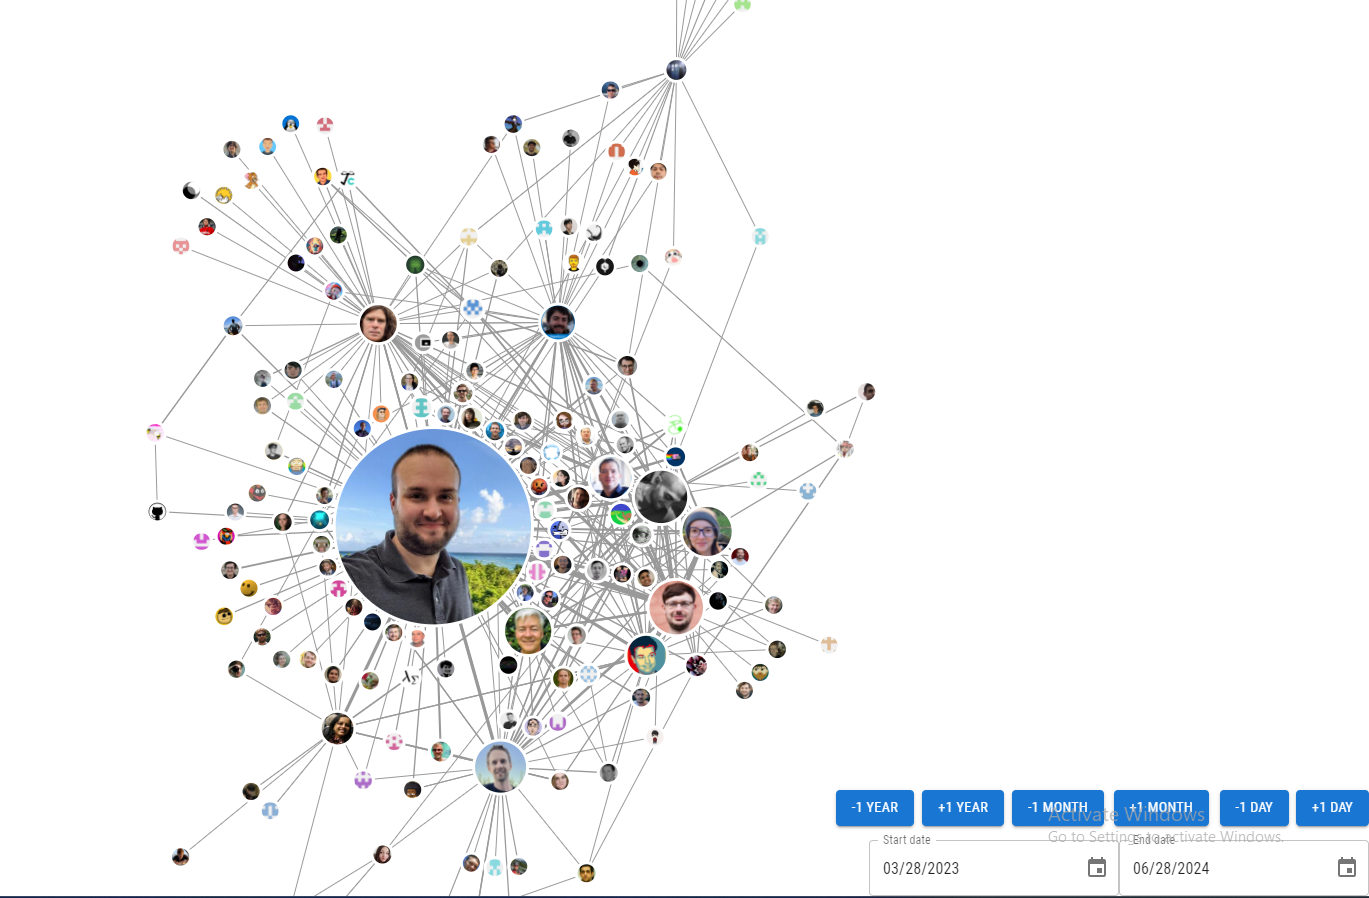
\includegraphics[width=8cm]{final-product}
    }
    \caption{\label{fig:final-product} Project prototype screenshot image.}
\end{figure}